%%% LSSTC_proposal.tex --- 

%% Author: ycao@Capricornus.local
%% Version: $Id: LSSTC_proposal.tex,v 0.0 2016/11/28 03:56:56 ycao Exp$

%%\revision$Header: /Users/ycao/workroom/projects/ZTF_marshal/Proposals/LSSTC/LSSTC_proposal.tex,v 0.0 2016/11/28 03:56:56 ycao Exp$

%%%---------------------------------------------------------------------

\documentclass[11pt]{article}
\usepackage[letterpaper, portrait, top=1in, bottom=1in, left=1in, right=1in]{geometry}
\usepackage{fancyhdr}
\usepackage{lastpage}
\usepackage{graphicx}
\pagestyle{fancy}
\lhead{\textbf{Transient Facebook}}
\rhead{\textbf{}}
\cfoot{\thepage/\pageref{LastPage}}
\usepackage{multicol}
\usepackage[font=small, labelfont=bf]{caption}
\usepackage{wrapfig}
\usepackage[shortlabels]{enumitem}
\usepackage{amssymb}
\usepackage{amsmath}
\setlength{\multicolsep}{2.0pt plus 2.0pt minus 1.5pt}
\usepackage{url}



\begin{document}

%%%%##########################################################################

\begin{center}
  \textbf{\Large Transient Facebook}\\
  Last Update: \today
\end{center}

\section{The Problem}
\label{sec:problem}

Astronomy is transforming from a data-starved to data-swamped
discipline. Data to be accumulated by next-generation astronomical
surveys, such as Zwicky Transient Facility (ZTF), Large Synaptic
Survey Telescope (LSST), and Wide Field Infrared Survey Telescope
(WFIRST), will expectedly exceed the total volume of existing data by
orders of magnitude. Particularly in the field of transients, ZTF,
which will start its survey within a year, is going to deliver $10^5$
events per night, while LSST is expected to send out $10^6$ event
alerts per night after the year 2022. 

Follow-up observations for classification and detailed
characterization of discovered transients have equally important
scientific values as discoveries. However, given the limited telescope
resources around the globe, not only will filtering events to select
interesting candidates for follow-up observations become essential,
but orginazation and coordination of follow-up observations as well as
follow-up data sharing imposes another challenge to researchers and
the community as a whole. For instance, fast-evolving transients (such
as orphan GRB afterglows, electromagnetic counterparts of
gravitational events) require rapid and intensive follow-up
observations within the first 24 hours of discovery. Distant
transients or late-time transients need big mirrors to observe.
Obviously, traditional methods such as emails and phone calls are not
sufficient to handle organization of timely follow-up observations of
such large numbers of alerts.


\section{Transient Facebook}
\label{sec:proposal}

Inspired by popular social media, in which people from all over the
world make friends, form groups, make requests and communicate
information, we propose a ``Transient Facebook'' system as a data
center for transients, an information center for follow-up requests,
and a workplace for individuals and collaborations. The main
funcionalities of ``Transient Facebook'' includes:
\begin{itemize}
\item Users can register a transient by its coordinates and create a
  ``Facebook'' page for it. The registration procedure does not depend
  on transient alerts from any specific survey. However, it will check
  whether a transient has been registered or not.

\item For a registered transient, ``Transient Facebook'' provides
  application program interaces (APIs) for users to upload relevant
  data at any time. The relevant data includes archival and follow-up
  data.

\item ``Transient Facebook'' visualizes uploaded data and provides
  basic analysis tools, such as light curve fitting, spectral matching
  and spectral line identification.

\item ``Transient Facebook'' allows users to post formal and informal
  analysis and comments on the transient ``Facebook'' page,
  facilitating communications and potentially fast publications.

\item ``Transient Facebook'' provides APIs for users to share
  information about their telescope times with
  collaborators. Collaborators then will be able to send observation
  requests about particular transients to observers.

\item ``Transient Facebook'' provides easy APIs for Users to download
  data of transients for further analysis.
  
\item ``Transient Facebook'' provides a basic search function
  for users to query transients based on their locations and types.

\item ``Transient Facebook'' will design a user adminnstration system
  to manage users and collaborations. Users will have privileges to
  decide how to share their data and postings to others within or
  outside collaborations.

\end{itemize}

\subsection{Relations With Other Tooling In Development}

The ``Transient Facebook'' provides a downstream tool for
investigating transients. In the upstream, the transient discovery
pipelines process survey data and produce transient alerts (such as
ZTF IPAC image differencing pipeline and LSST Level 1 products). In
the midstream, a broker annotates these alerts within information from
external sources and a cascade of filters to select interesting
candidates (ANTARES in LSST). In the downstream, interesting
transients with all available data are collected in the ``Transient
Facebook'' which provides a one-stop station to organize further
observations and analysis.

\section{Prototype: PTF Marshal System}
\label{sec:marshal}

Since 2009, the Palomar Transient Factory (PTF) has been using a prototype
``Transient Facebook'' called ``Marshal'' within its collaboration. Experience
has shown that ``Marshal'' has greatly improved efficiency in communication,
organization and publication within the PTF collaboration. Figures \ref{fig:sn2011fe_overview}
to \ref{fig:sn2011fe_spec} shows screenshots of ``Marshal'' pages for PTF11kly
(SN2011fe). 

\begin{figure}[htb]
  \centering
  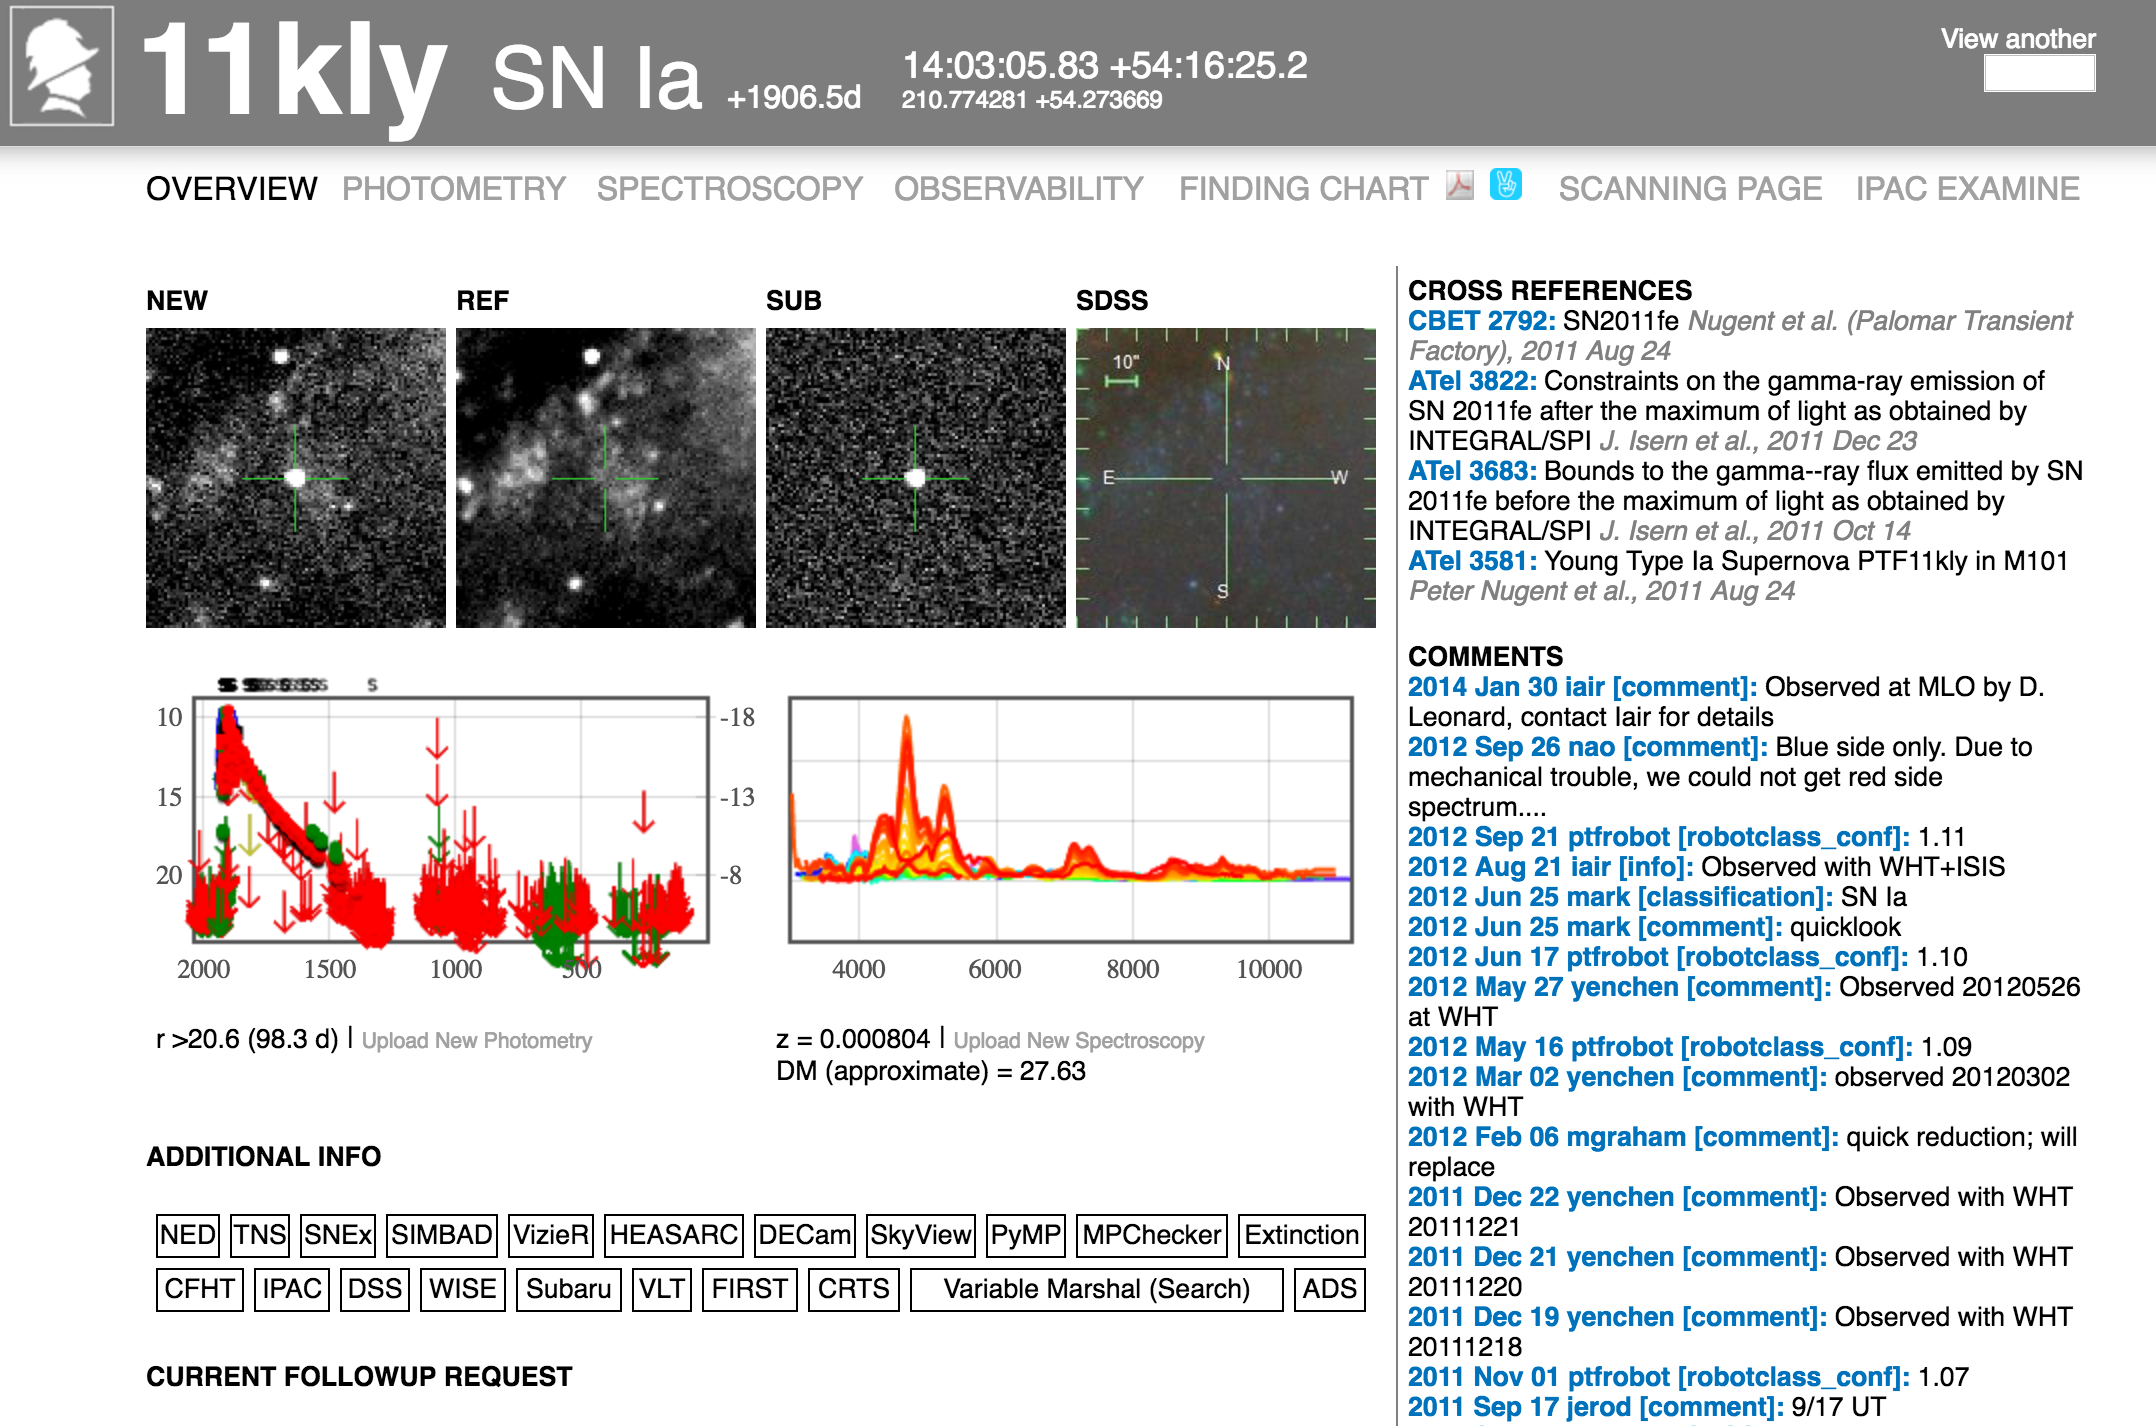
\includegraphics[width=0.8\textwidth]{view_source.png}
  \caption{Screenshot of ``Marshal'' overview page of PTF11kly (SN2011fe)}
  \label{fig:sn2011fe_overview}
\end{figure}

\begin{figure}[htb]
  \centering
  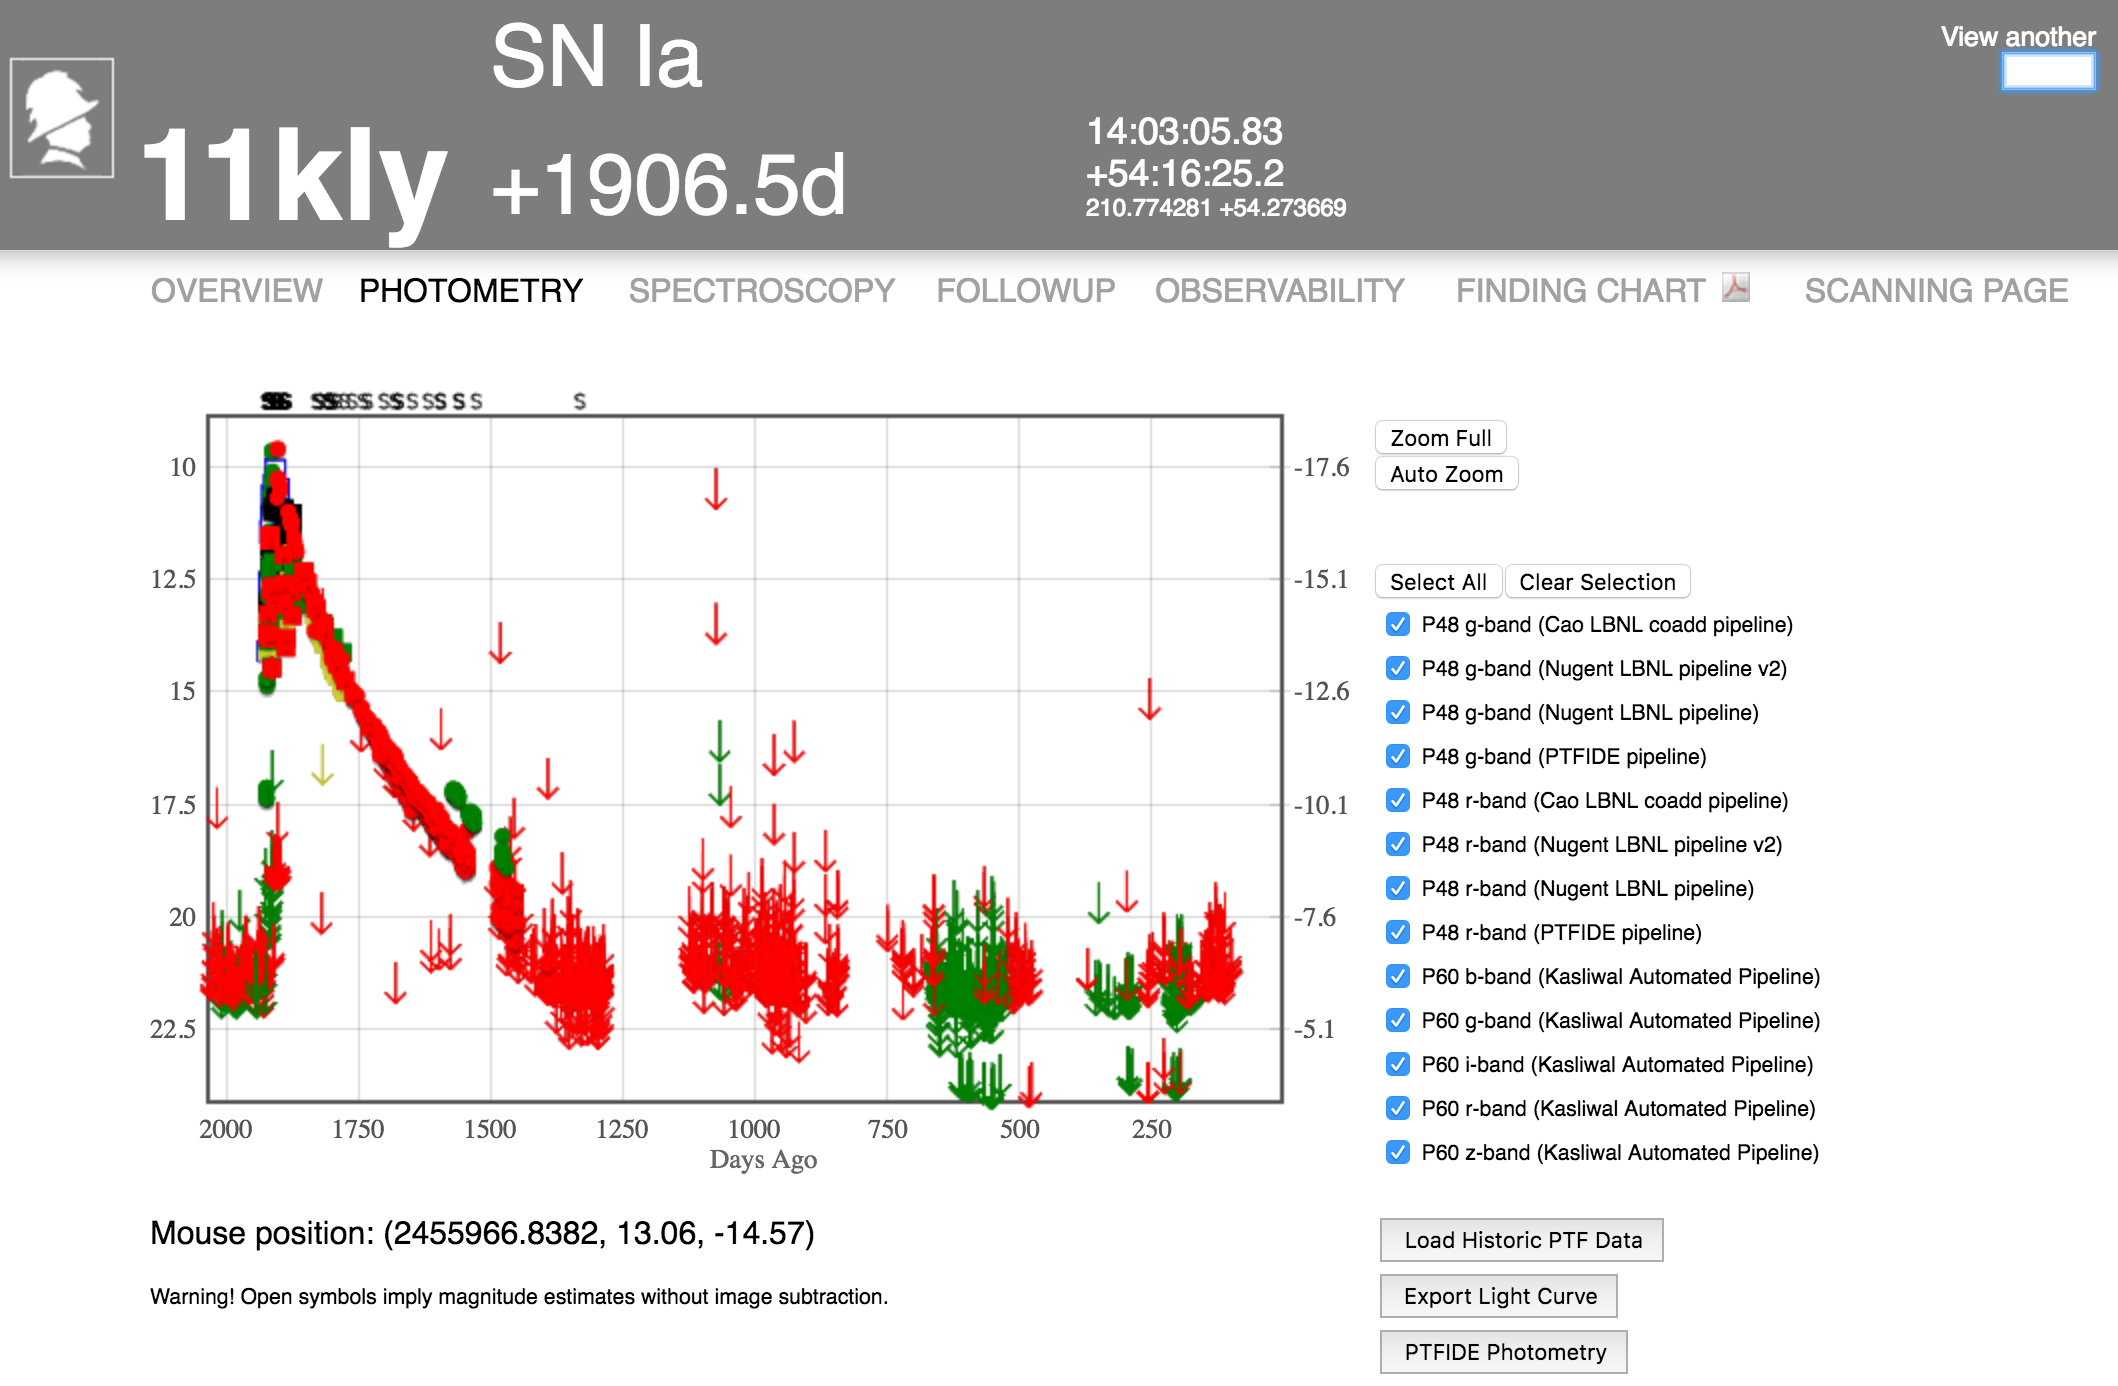
\includegraphics[width=0.8\textwidth]{plot_lc.png}
  \caption{Screenshot of ``Marshal'' light curve page of PTF11kly (SN2011fe)}
  \label{fig:sn2011fe_lc}
\end{figure}

\begin{figure}[htb]
  \centering
  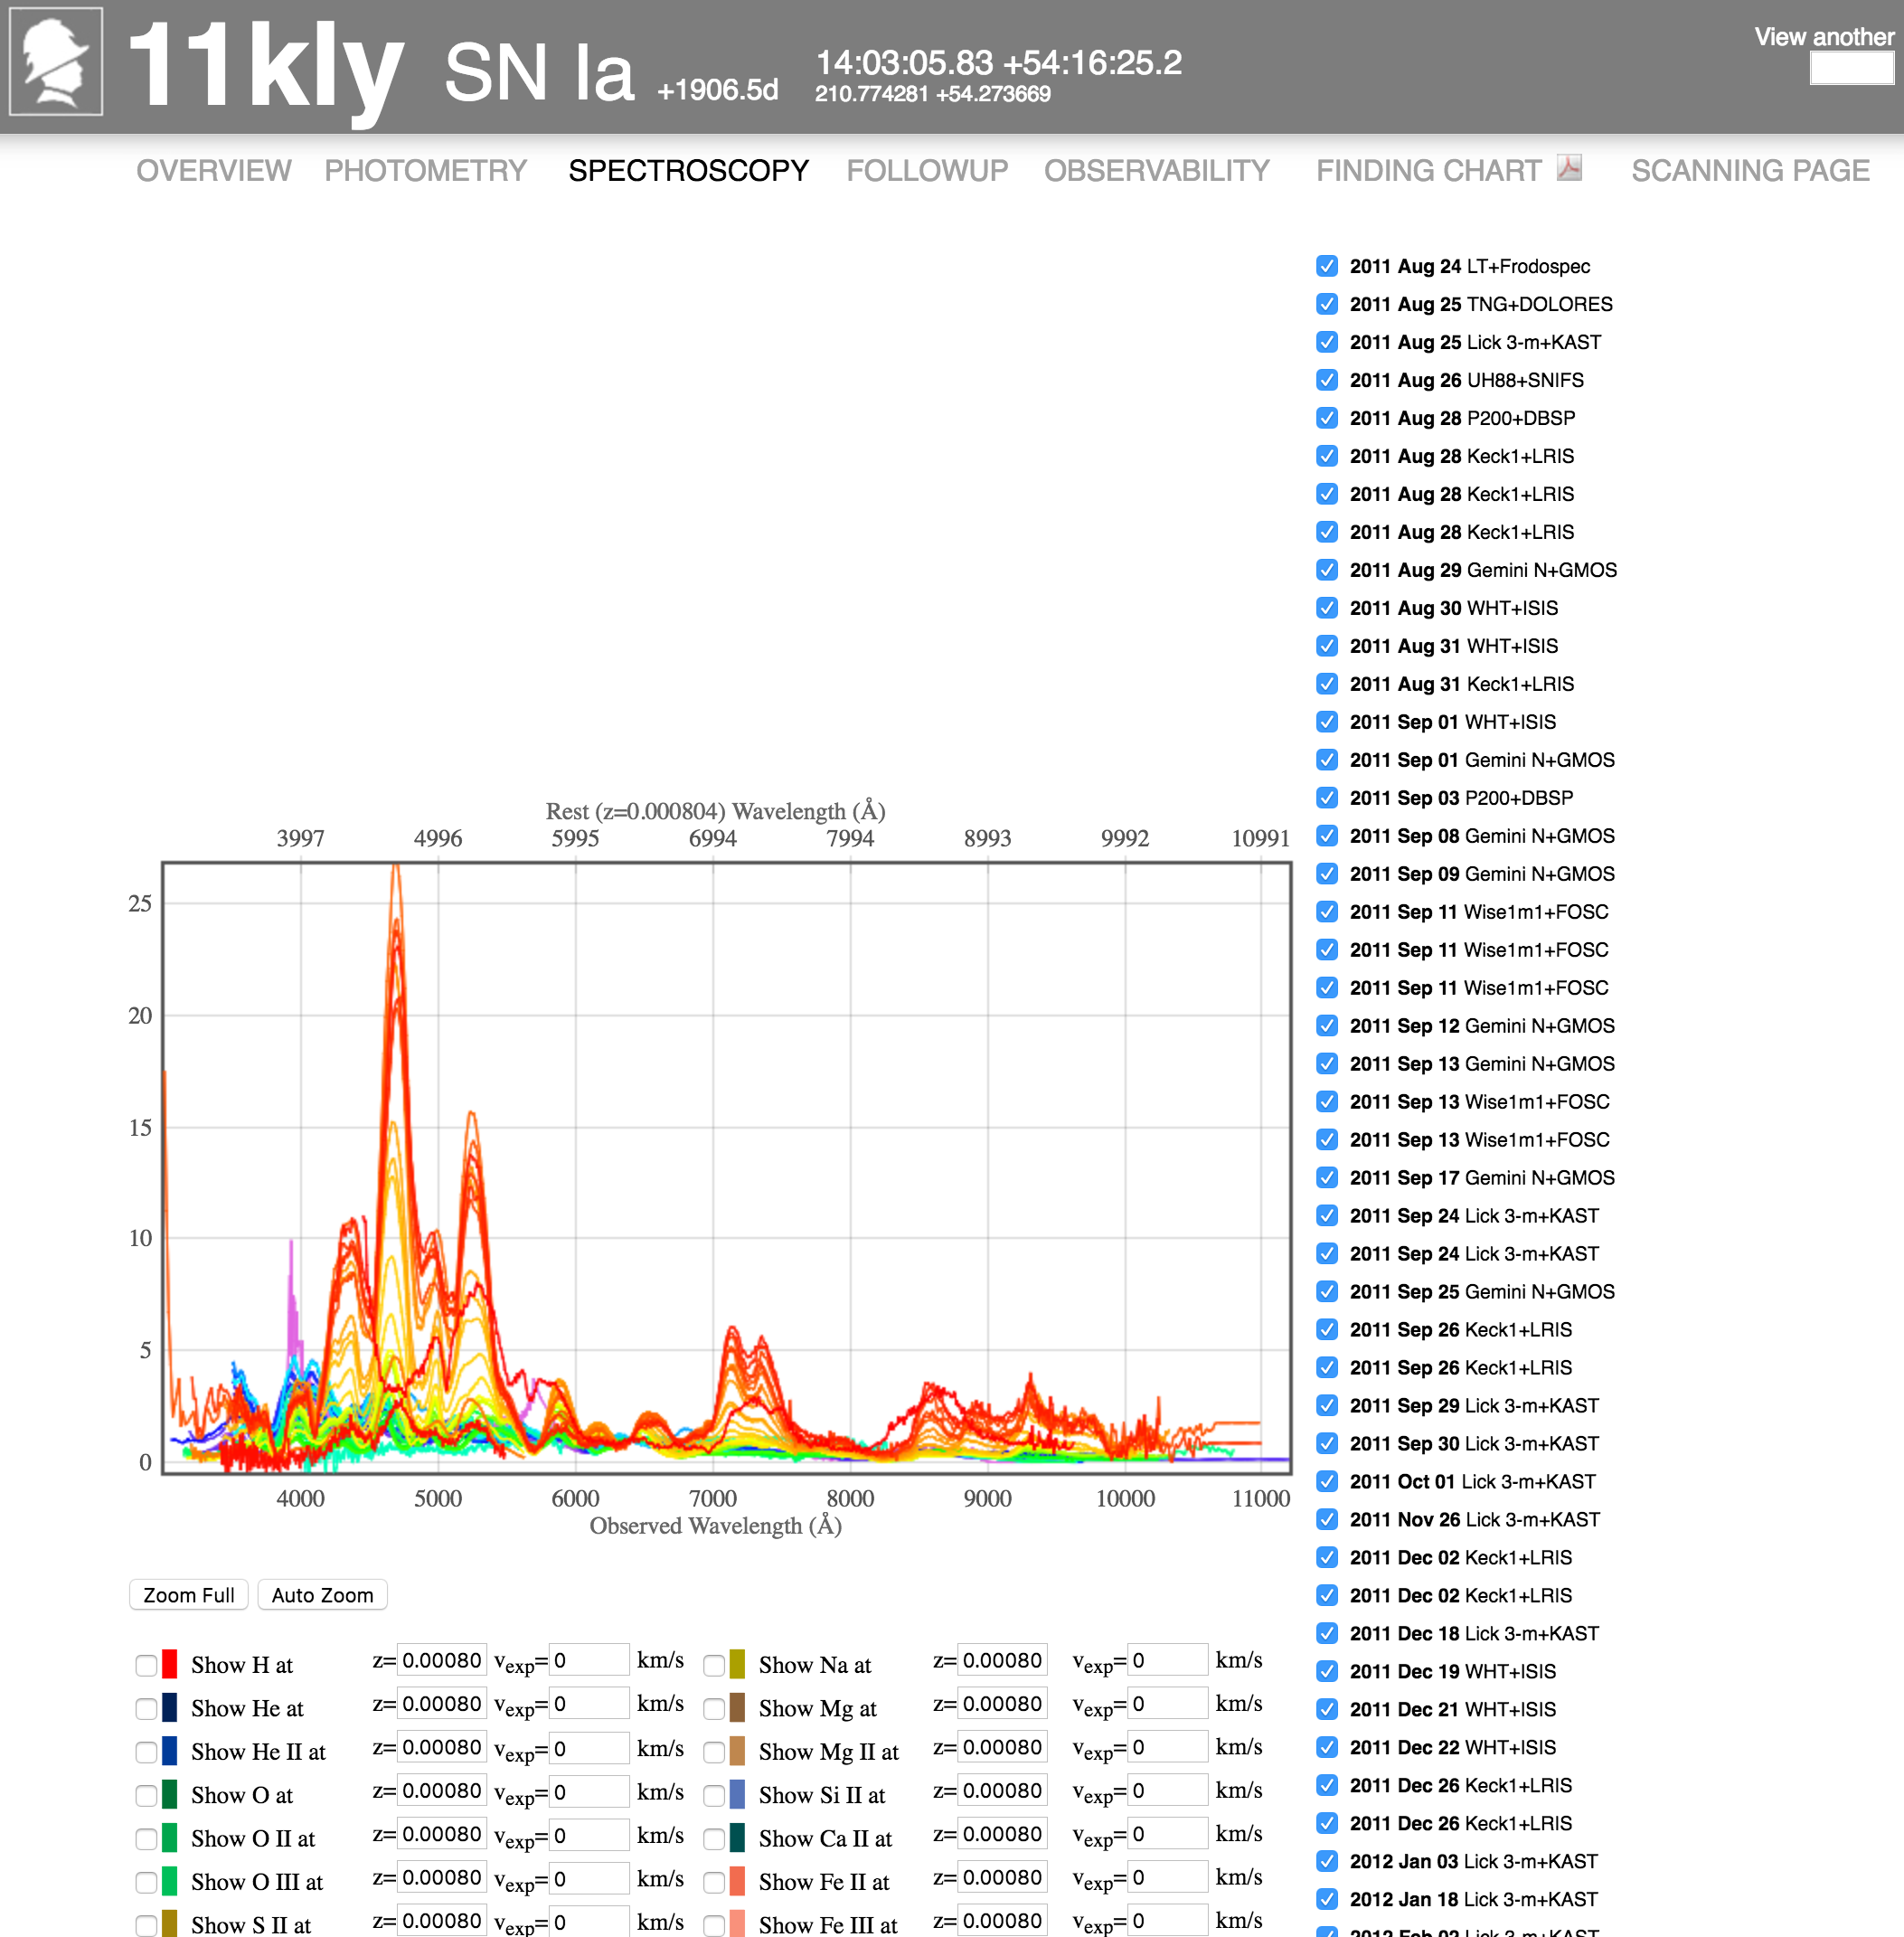
\includegraphics[width=0.8\textwidth]{view_spec.png}  
  \caption{Screenshot of ``Marshal'' spectral page of PTF11kly (SN2011fe)}
  \label{fig:sn2011fe_spec}
\end{figure}

The ``Marshal'' system was designed to match the discovery rate of
PTF. The technologies behind it, including backend database and
frontend web server, were also outdated. As a result, the whole system
is not scalable to meet the data challenges in ZTF and LSST.

\section{Requests}
\label{sec:request}

Based on the prototypical PTF Marshal system, we request funding in
support of developing the ``Transient Facebook'' software system. The
upcoming ZTF project (which is scheduled to run between mid-2017 and
mid-2020) with an unprecedentedly large rate of transient discovery
provide an apropriate testbed for the ``Transient Facebook'', before
LSST comes online.

Specifically, we ask for money in the next three years for the following items
\begin{itemize}
\item Salary for personnels to develop and improve the ``Transient Facebook''
  system.
\item Purchases of computing resources to run the system either on local machines or
  on commercial clouds. 
\item Conferences and workshops to introduce the ``Transient
  Facebook'' system to the community.
\end{itemize}
The total amount is TBD. 


%%%%##########################################################################

\end{document}
